\graphicspath{{figures/chapter-intro/}} % Specifies the directory where pictures are stored


\chapter{Introduction}
\label{cha:intro}


Anthropogenic climate change has been a hot topic amongst scientists and the public for the past decade. A few of the primary questions associated with climate change relate to how scientists know that climate change is caused by humans and where and when the effects of climate change will be seen. Both of these questions require an understanding about what causes the climate to change over time. Earth's climate is a complex dynamic system and has changed constantly throughout Earth's history. Being able to separate the climate's natural fluctuations from the change caused by anthropogenic activity is essential to being able to accurately predict and detect future changes in climate.

\section{Natural Variability}

One of the primary challenges of assessing the impact of anthropogenic influence on Earth's climate is a lack of understanding of the natural fluctuations of the climate system. Internal climate variability is simply how Earth's climate varies in time without any external forcing. External forcing can be natural in source, including volcanic eruptions, and solar forcing, or anthropogenic, including human emissions of greenhouse gases and human caused land use changes. The term natural variability on the other hand is typically used to refer to fluctuations in Earth's climate caused solely by natural forcing (internal or external), and not including anthropogenic influence.

Natural variations in the climate system, also referred to as 'climatic noise', (Madden, 1976; Schneider and Kinter, 1994; Wunsch, 1999; Feldstein, 2000) are a result of non-linear dynamical and biological processes in the atmosphere and ocean operating on a variety of spatial and temporal scales. The most common example of natural variability is the El Ni\~no-Southern Oscillation (ENSO), which is a result from the non-linear interactions between the atmosphere and ocean in the Equatorial Pacific. While ENSO is perhaps the most famous of all the atmospheric climatic modes of variability, there are multiple modes of variability in the atmosphere and ocean which interact with each other.

A further complicating matter is that climate variations happen on all timescales: paleo-climatic, centennial, multi-decadal, decadal, inter-annual, and seasonal, in addition to on all spatial scales from regional to global. Global variability on long timescales is generally the best understood, however regional variability is generally the most important when it comes to understanding and interpreting recent trends in observational data.

Quantification of natural variability is important to climate science for many reasons. First, natural variability is key to determine climate predictability. Climate predictability was first defined in 1975 (Academy of sciences publication, 1975) as a measure of signal-to-noise, where the signal is any potentially predictable long-term (> 1 year) climate feature, and the noise is natural variability. Having an estimate of natural variability allows us to answer the question - how large does a trend need to be in order to detect it? Without an idea of what the natural variability of a given feature is, it is nearly impossible to determine if a signal lies within the noise of the climate system.
Another reason quantifying natural variability is important relates to projection uncertainty. Characterizing uncertainty for climate change projections is important for purposes of detection and attribution and for strategic approaches to adaptation and mitigation (Deser et al, 2012). Uncertainty in future climate change comes from three main sources: forcing, climate model response, and internal variability (Lovenduski et al 2015, Hawkins and Sutton 2009; Tebaldi and Knutti 2007).

A final example of where understanding natural variability is important is in the evaluation of global climate models. Because of observational limitations and the inability to experiment on the entire earth system, climate models are developed and used to further our knowledge of the planet and climate system. Climate models are typically validated against the mean state of a given climate feature. For example, to assess the accuracy of the ocean module in a climate model, one might compare the average sea surface temperature (SST) in a pre-industrial control model run to the average of many years of SST observations from similar period (via proxy records). While this method is useful for assessing the mean state of the climate model, it does not give any information about the variability of the model. The model could have vastly larger variance than the observations, which would not be captured by comparing the means.
One of the largest challenges with estimating natural variability is a lack of observational estimates. In an ideal situation, scientists would be able to quantify natural variability using observations of the Earth system. However, because natural variability operates on all time and spatial scales, this would require millions of observations across the entire globe. Global natural variability over thousands of years is estimated using proxy records of Earth's climates; however, regional variability on shorter timescales (decadal to multi-decadal) is much more of a challenge to quantify because it requires finer resolution of observations.

To supplement the limited observational estimates of natural variability, scientists often turn to global climate models to quantify natural variability. Unlike observational records, global climate models have a consistent spatial and temporal resolution. Global climate models can also be used to simulate multiple realizations of Earth's climate over thousands of years, to generate a statistical distribution of climate variability in absence of external forcing. Because no single climate model is a perfect representation of Earth's dynamical and biological processes, multiple models are often employed to reduce the uncertainty due to model configuration. This method of quantifying natural variability also comes with challenges. Primarily, global climate models are very computationally expensive and require extensive resources and time to generate a simulation. Additionally, to best quantify natural variability, multiple simulations without any anthropogenic forcing should be performed. Because of the emphasis on simulating future change, fewer resources have traditionally been put toward conducting non-anthropognically forced simulations.

In this thesis, natural variability in both physical fields (winds and temperature) and biogeochemically active fields (carbon and oxygen) is examined across multiple scales.


\section{Thesis Overview}
This thesis takes an investigative look at the multi-decadal natural variability of three important components of the climate system: the Southern Hemisphere westerly jet, oceanic carbon and heat content, and North Atlantic oxygen and age. These three components of the atmosphere and ocean variability were selected because of the important role they have in the response of the global climate system.

\subsection{Chapter 2 - Southern Hemisphere Westerly Jet}
The Southern Hemisphere (SH) westerly jet is incredibly important for driving the Southern Ocean circulation, which has strong influence on global climate. The strong, eastward flowing winds of the drive subsurface Ekman transport towards the north. This northward flowing water is colder than the water it encounters (and therefore denser) and subsequently sinks into the interior to form Antarctic Intermediate Water - a process known as ventilation. Closer to the Antarctic continent, overlaying easterly winds drive the surface water towards the south where waters interact with the Antarctic sea ice and dense water is formed (formation of Antarctic Bottom Water). The resulting divergence of water at the surface of the Southern Ocean allows for deep water (primarily North Atlantic Deep Water) to rise to the surface and interact with the atmosphere (Figure 2).

This process of water rising to the surface, interacting with the atmosphere, and subsequently sinking back into the interior allows for increased atmosphere-ocean gas exchange and results in the Southern Ocean being very influential on global climate. the Southern Ocean is one of the most important oceans for regulating global climate. Recent estimates suggest that the Southern Ocean is responsible for 75\% of the heat uptake and 30\% of the carbon uptake (Frolicher et al 2014)

Recent studies suggest that anthropogenic ozone depletion and greenhouse gas induced warming has already had an impact on the SH westerly jet through a strengthening and shift towards the Antarctic continent. In this Chapter 2, we utilize 14 state-of-the-art global climate models from modeling centers around the world to quantify the natural variability in the SH westerly jet. We then compare the model-estimated natural variability to the recently observed trends in the jet strengthening and pole-ward shift. Our results suggest that a combination of natural variability and anthropogenic forcing are required to explain the observed trends in the SH westerly jet.

\subsection{Chapter 3 - Oceanic Heat and Carbon Variability}
Chapter 3 turns to the role of natural variability in the Southern Ocean on the global and regional oceanic heat and carbon budget. One particular phenomenon that holds significant implications for global climate is deep ocean convection. The high-latitude Southern Ocean is weakly stratified with cold fresh water overlaying slightly warmer saliter water of nearly identical density (Martinson, D. G., 1991). Deep convection in this region occurs when this weakly stratified surface layer is perturbed and becomes denser than the under-laying waters resulting in the entire water column turning over. This results in the surface waters being subducted deep into the ocean, and old deep water being brought up to the surface.

While only one of these deep convective events have been observed in the real Earth's Southern Ocean (the Weddell Polynya which persisted through the winters of 1974-1976) many global climate models have consistent periodic convection events in this region (deLavergne et al.). Because of the intense exchange of surface and deep waters associated with deep convection, these events have been shown to have profound impacts on global climate (Gordon, A. L 1982, Cabre et al).

In Chapter 3, we use multiple simulations from a coarse-resolution climate model to explore the temporal variability of oceanic carbon and heat and investigate how this global heat and carbon variability is impacted by Southern Ocean deep convective events. We show that the Southern Ocean deep convection has significant influence on the magnitude of global oceanic heat and carbon variability, however the relationship between oceanic heat and carbon remains consistent with varying convection.

\subsection{Chapter 4 - Age and Oxygen Relationship}
Chapter 4 builds on this idea that biological and physical responses to changes in circulation may differ. Oceanic age refers to the time since the ocean water was last in contact with the atmosphere. This derived tracer is used to estimate the rate of ocean ventilation and overturning circulation. Oxygen is another tracer that is important to understanding ocean circulation and biological activity. Age and oxygen are generally thought to have a strong negative correlation because biological utilization reduces oxygen concentrations in the ocean interior where the age is the oldest. This presumed relationship is often times used in ocean biogeochemistry and oceanography to estimate changes in biological activity and ocean circulation.

We focus on an observational data set in the North Atlantic and look at how changes in oxygen and oxygen utilization relate to changes in ventilation age. We show that in the observational record and in a global climate model simulation, along Line W in the North Atlantic this expected relationship between age and oxygen is more complicated due to the different spatial structure of sources of apparent oxygen utilization and age in the deep ocean.


\begin{figure}
\centering
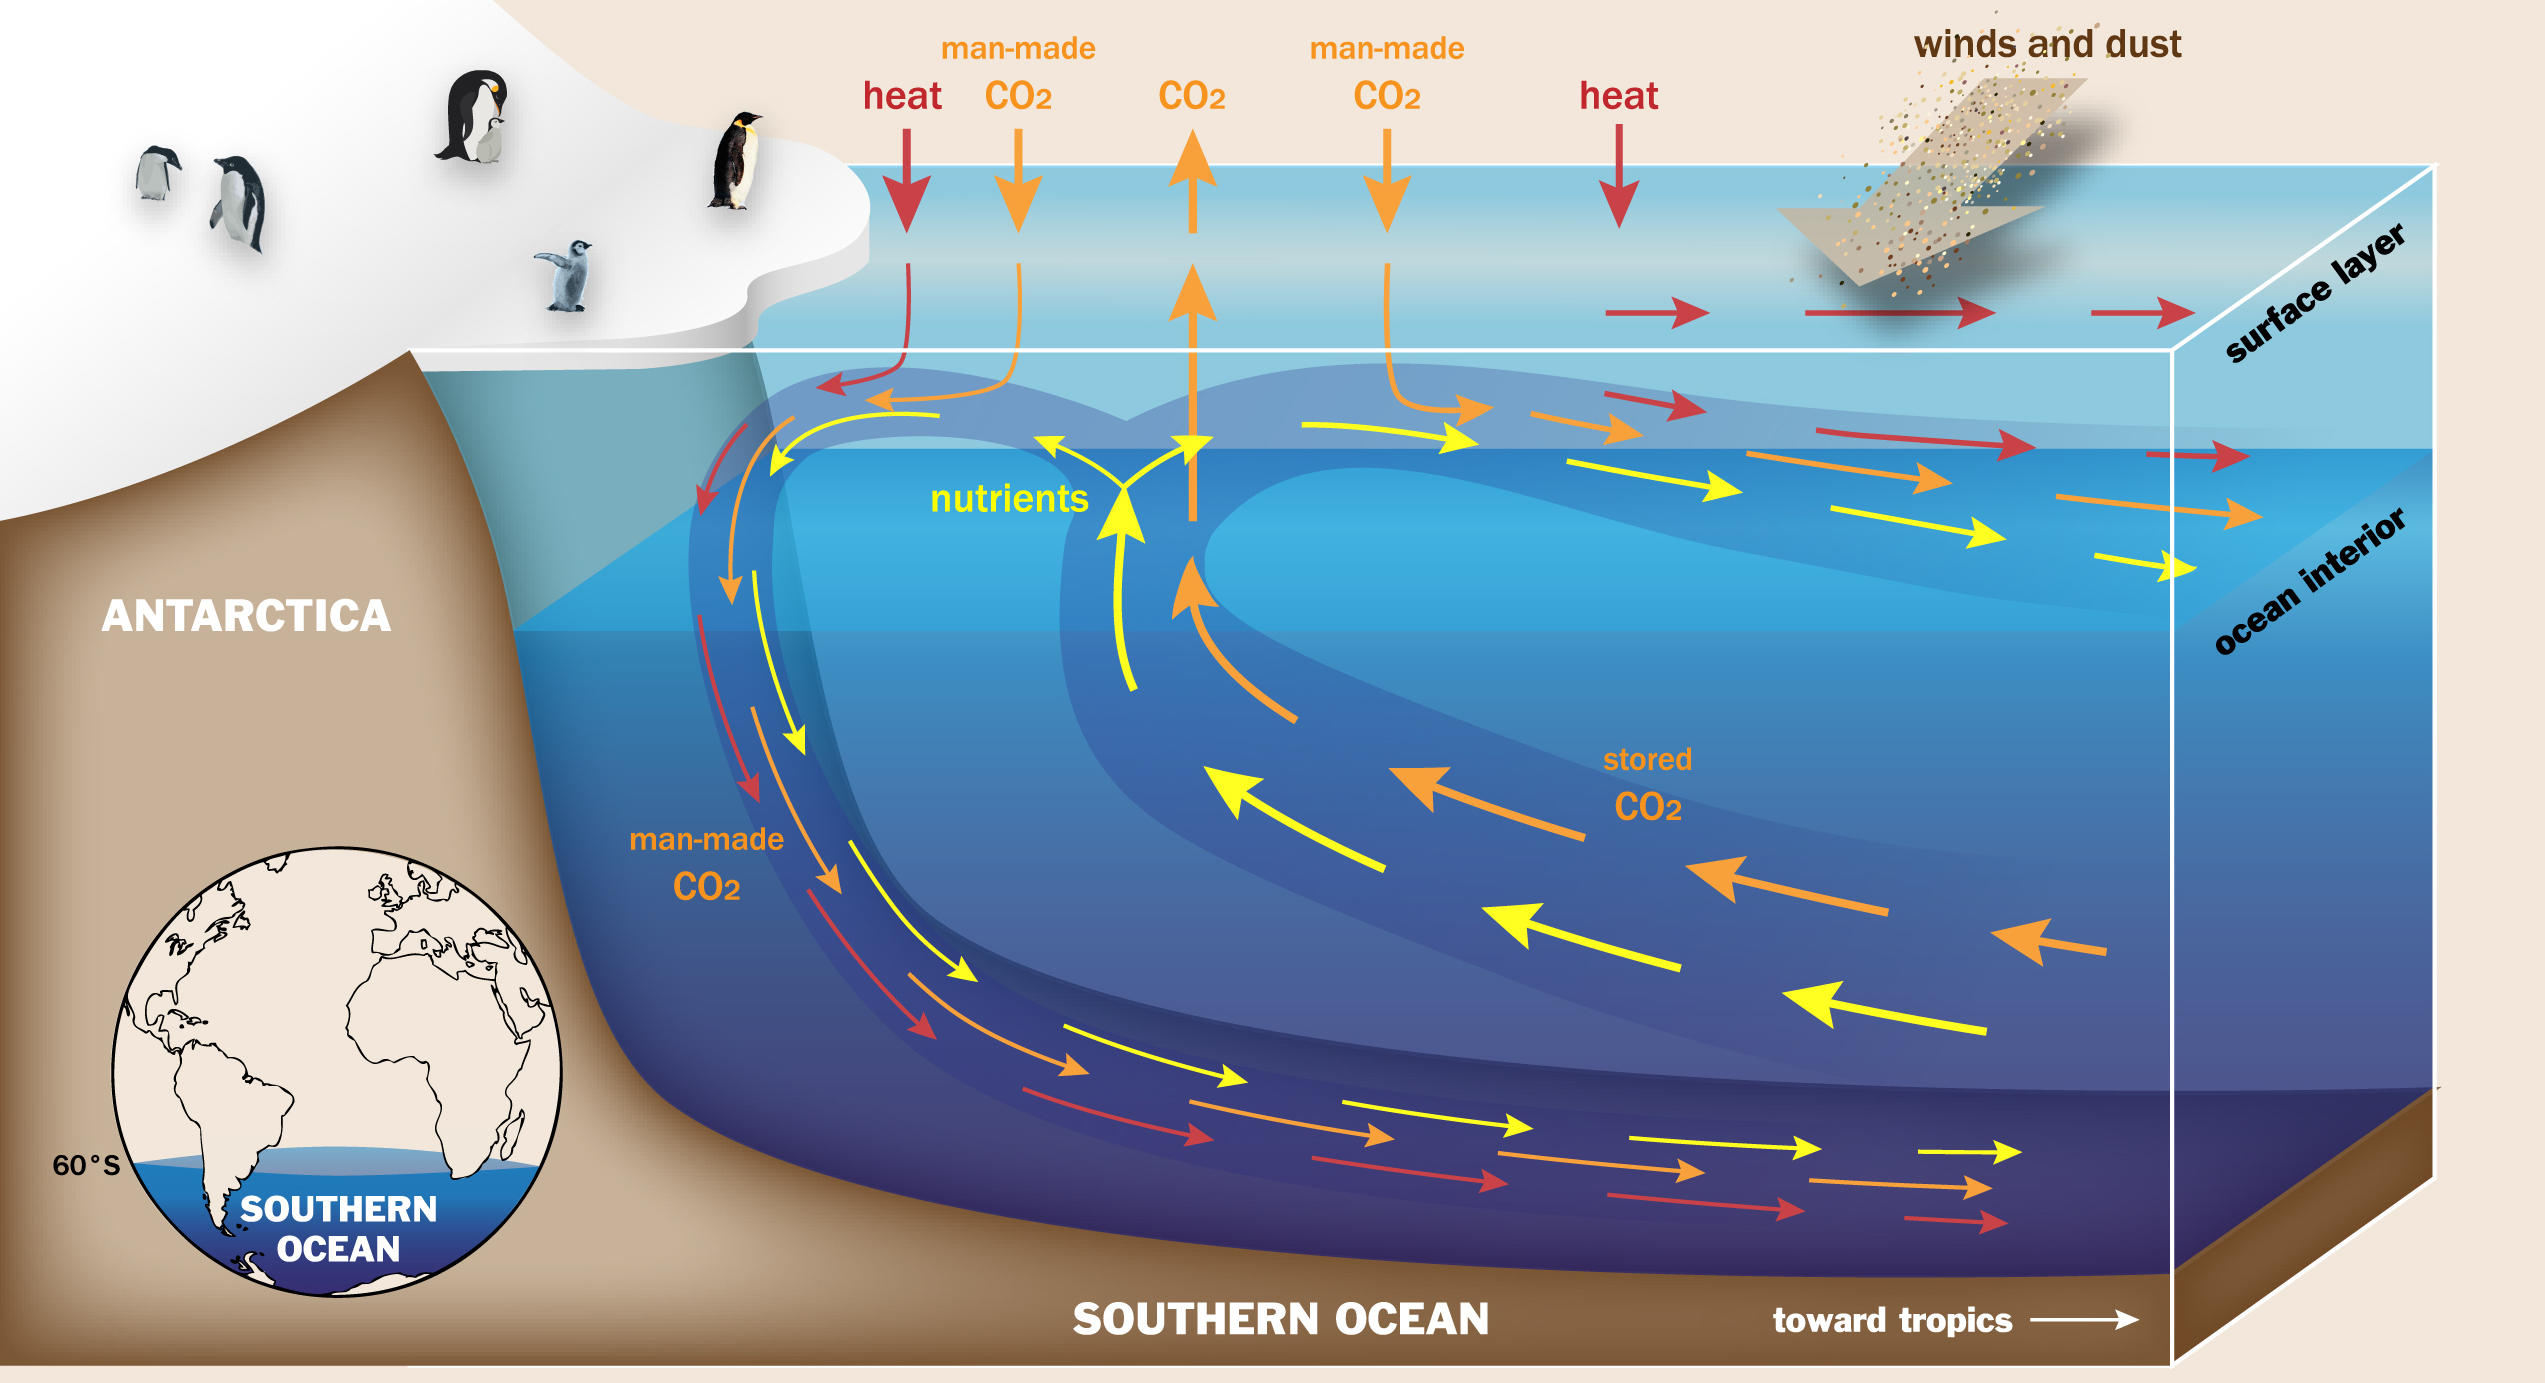
\includegraphics[width=33pc]{Southern_Ocean.jpg}
\caption{Schematic depicting Southern Ocean circulation. Figure by Ilissa Ocko, courtesy of Princeton University.}
\label{fig:carbon_cycle}
\end{figure}


%%% Local Variables:
%%% mode: latex
%%% TeX-master: "thesis"
%%% End:
